\documentclass[11pt,table,t]{beamer}

% Packages
\usepackage{xcolor}
%\usepackage{eulervm}
\usepackage[norsk]{babel}
\usepackage[utf8]{inputenc}
\usepackage{tabularx}
\usepackage{cancel}


% Theme
\mode<presentation>
{
  \usetheme{Honefoss}
%  \setbeamercovered{transparent}
  \setbeamertemplate{blocks}[rounded]
  \AtBeginPart{\frame[c]{\partpage}}
}

\newcommand{\comment}[1]{{\slshape\color{kvred}#1}}
\usebackgroundtemplate{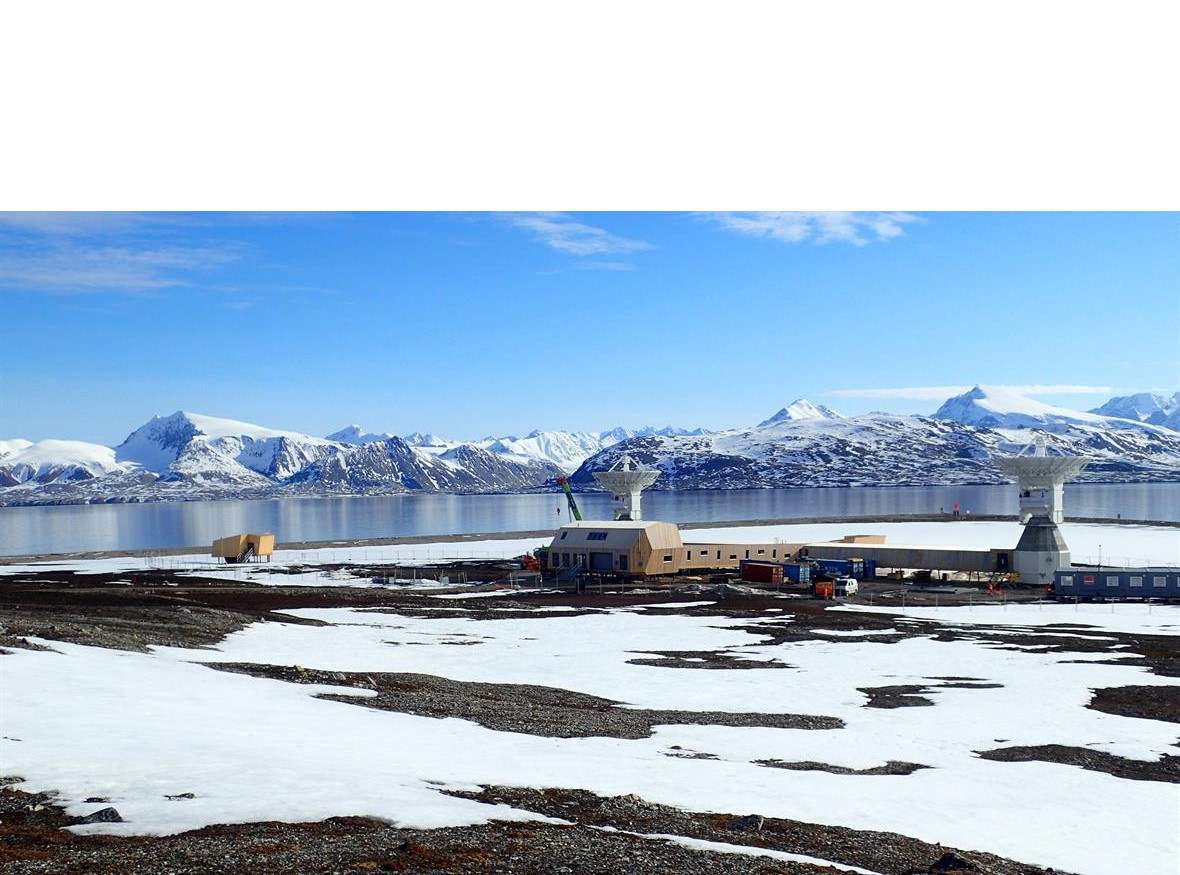
\includegraphics[width=\paperwidth]{figure/nyal_antennas}}

\title{Where}
\subtitle{-- high precision positioning using Python}
\author{Michael Dähnn, Ingrid Fausk, Geir Arne Hjelle, Ann-Silje
  Kirkvik, Eirik Mysen}
\date{EuroSciPy, August 25 2016}
%\titlegraphic{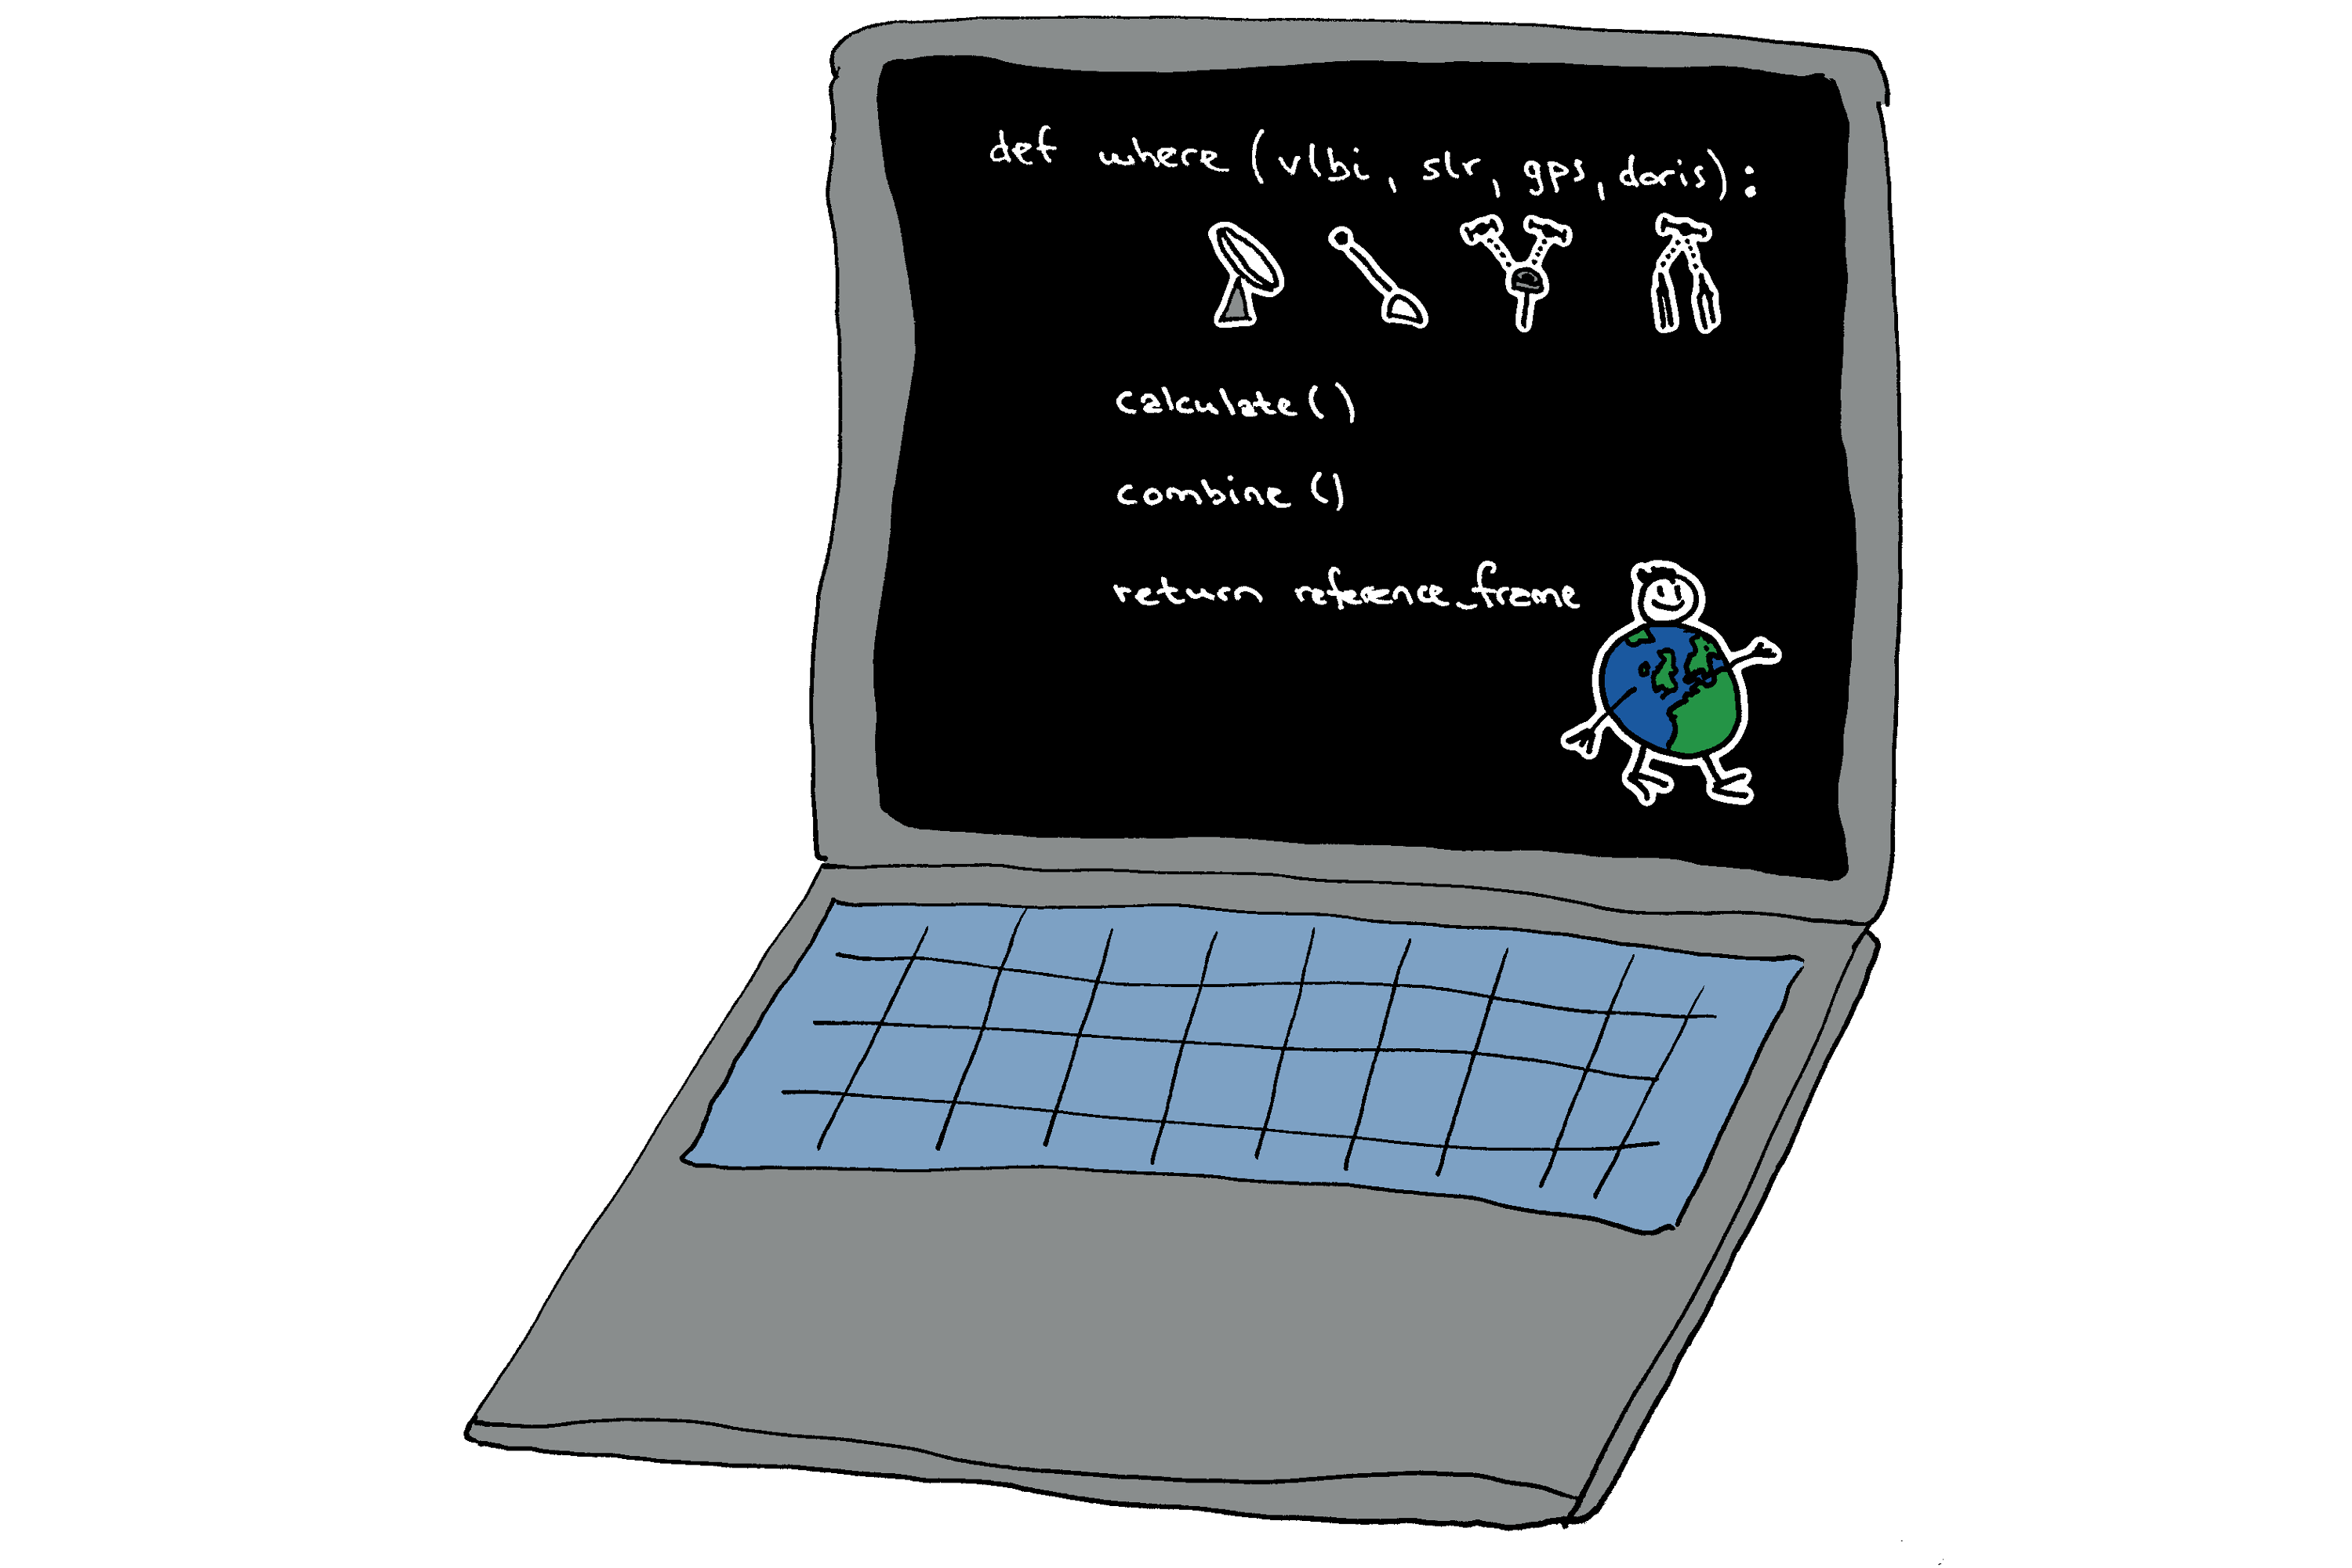
\includegraphics[width=\paperwidth]{figure/where}}

\begin{document}

\begin{frame}{Where -- High Precision Positioning using Python}

  The Norwegian Mapping Authority is currently upgrading the geodetic station at
  Ny {\AA}lesund, $79^\circ$ north.

  \medskip
  Quasars, lasers and satellites are used to determine positions at the
  millimeter level. This is important for better climate monitoring, improved
  satellite systems and new positioning technologies.

  \vspace*{4.2cm}

  %\color{kvgreen}
  We are writing new software for doing this analysis, in Python.
\end{frame}

\end{document}
